\chapter{Development of a Web Application Programming Interface for Genome 
Properties Data} \label{micromeda-server}

As discussed in Chapter \ref{introduction}, one of the goals of Micromeda is to 
provide users with an interface for visualizing the presence and absence of 
genome properties across multiple organisms. Users can access Micromeda's heat 
maps through a web application that generates them from uploaded Micromeda file 
data. The use of a web application has several advantages that are discussed in 
Subsection \ref{why-micromeda-files}. Micromeda's web application consists of 
two components: client and server. The \gls{ui} client, which draws the heat 
maps, is supported by a web server process that parses Micromeda files and 
provides a web \gls{api} for accessing these file's contents. This chapter will 
discuss the server component of Micromeda, called Micromeda-Server, including 
the services it provides and its implementation. The client web application that 
uses these services is discussed in Chapter \ref{micromeda-client}. Source code 
for Micromeda-Server is located at 
\href{https://github.com/Micromeda/micromeda-server}{github.com/Micromeda/micromeda-server}.

\section{Overview of Web Servers} \label{web-servers}

The World Wide Web and associated web applications are ideal delivery mechanisms 
for data analysis software such as Micromeda \cite{berners1994world}. Such 
applications follow a client-server architecture \cite{svobodova1985client} (see 
\href{http://en.wikipedia.org/wiki/Client-server_model}{en.wikipedia.org/wiki/Client-server\_model}) 
where the code running in the user's browser is called the client. The user 
acquires this client by downloading it into their browser like any other 
webpage. If the client requires external data, then it can request this 
information from a server process running on a server computer 
system\footnote{For the rest of the thesis, the term \textbf{server computer 
system} is used to refer to the physical hardware on which server software is 
run. The term \textbf{server} is used to refer to a software process that 
provides users or applications with data.}. Requests to the server are made, via 
\gls{http} \cite{fielding1999hypertext}, using a series of \gls{url} addresses 
\cite{berners1994rfc} (\textit{i}.\textit{e}., web addresses) that return 
specific types of data. These addresses are known as \textbf{endpoints} (Section 
\ref{endpoints}) and form a web \gls{api}.

\section{Micromeda-Server Workflow and Implementation} \label{server-workflow}

Micromeda-Server is designed to provide a web \gls{api} to client applications 
that require access to information about the Genome Properties database. The 
server also provides an \gls{api} for accessing temporarily stored property 
assignments, step assignments, and supporting information for user-supplied 
datasets. Micromeda-Server is written in Python and utilizes the Flask web 
development framework \cite{grinberg2018flask} (Fig. \ref{fig:micromeda-server}) 
to map Python functions for handling specific web \gls{api} requests to server 
\gls{url} addresses (\textit{i}.\textit{e}., ``endpoints"). Information about 
the Genome Properties database is supplied to Micromeda-Server via a 
\textbf{genomeProperties.txt} release file (Fig. \ref{fig:micromeda-server} and 
Subsection \ref{Genome-Properties-Files}). Property assignments, step 
assignments, and supporting information for user datasets are supplied via 
user-uploaded Micromeda files (Fig. \ref{fig:micromeda-server}). These Micromeda 
files are parsed into GenomePropertyResultsWithMatches objects (Subsection 
\ref{PropertyResultsWithMatches}) that are later stored in an in-memory Redis 
cache \cite{han2011survey} in MessagePack format \cite{furuhashi2013messagepack} 
(Fig. \ref{fig:micromeda-server}, Fig. \ref{fig:micromeda-server-workflow} and 
Section \ref{msgpack}). In the context of Micromeda-Server, the contents of each 
uploaded and cached Micromeda file is called a dataset. A single Micromeda file, 
stored on the same server computer system as Micromeda-Server, can also be 
provided to Micromeda-Server during start-up for use as a default dataset (Fig. 
\ref{fig:micromeda-server}). This default dataset is also parsed to a 
GenomePropertiesResultsWithMatches object and is used to supply data to 
Micromeda-Server's \gls{api} if users have not uploaded any Micromeda files. The 
standard workflow for starting and then using Micromeda-Server is the following:

\FloatBarrier
\begin{enumerate}
  \item Start Micromeda-Server while providing a \textbf{genomeProperties.txt} 
file and an optional default Micromeda file (Fig. \ref{fig:micromeda-server})
  \item The \textbf{genomeProperties.txt} file is parsed to a 
GenomePropertiesTree object
  \item The default dataset Micromeda file is parsed to a 
GenomePropertiesResultsWithMatches object  
  \item The client application sends a user-supplied Micromeda file to the 
server via the upload endpoint (Fig. \ref{fig:micromeda-server-workflow})
  \item The user-supplied Micromeda files are parsed to a 
GenomePropertiesResultsWithMatches object that is later stored in the Redis 
cache in MessagePack format (Fig. \ref{fig:micromeda-server-workflow})
  \item The server supplies the client with a dataset key that is unique to each 
uploaded Micromeda file (Fig. \ref{fig:micromeda-server-workflow})
  \item The client can later supply this dataset key to the server during 
proceeding \gls{api} requests to get information from the previously uploaded 
Micromeda file (Fig. \ref{fig:micromeda-server-workflow})
  \item If the client provides no dataset key then the server supplies 
information about the default dataset during \gls{api} requests
\end{enumerate}

\begin{figure}[!ht]
  \centering
	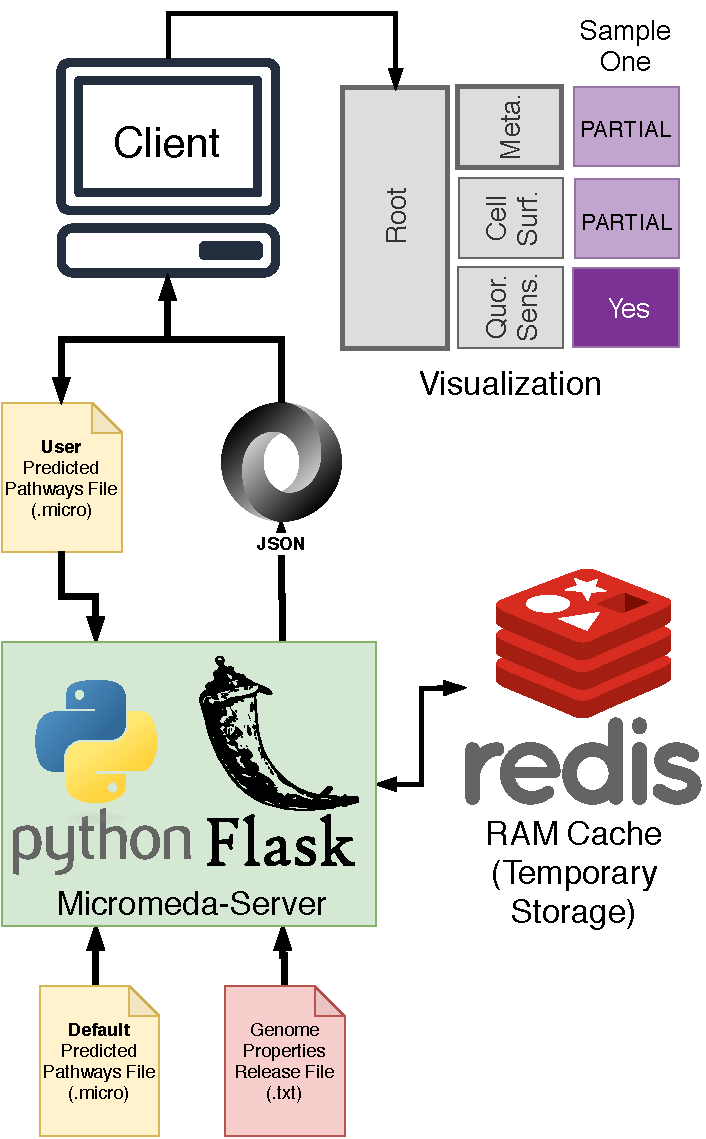
\includegraphics[width=0.58\textwidth]{media/Micromeda-Server.pdf}
	 \caption[Components of Micromeda-Server's software 
architecture.]{\textbf{Components of Micromeda-Server's software architecture.} 
The web server code was written in Python using the Flask web framework 
\cite{grinberg2018flask}. Micromeda-Server is supported by a Redis cache and a 
series of text files. A genomeproperties.txt file supplies data for the 
generation of Genome Properties \gls{dag}. Micromeda files, either default or 
uploaded, provide information about property assignments, step assignments, and 
supporting information of multiple organisms.}
	 \label{fig:micromeda-server}
\end{figure}

\begin{figure}[!ht]
  \centering
	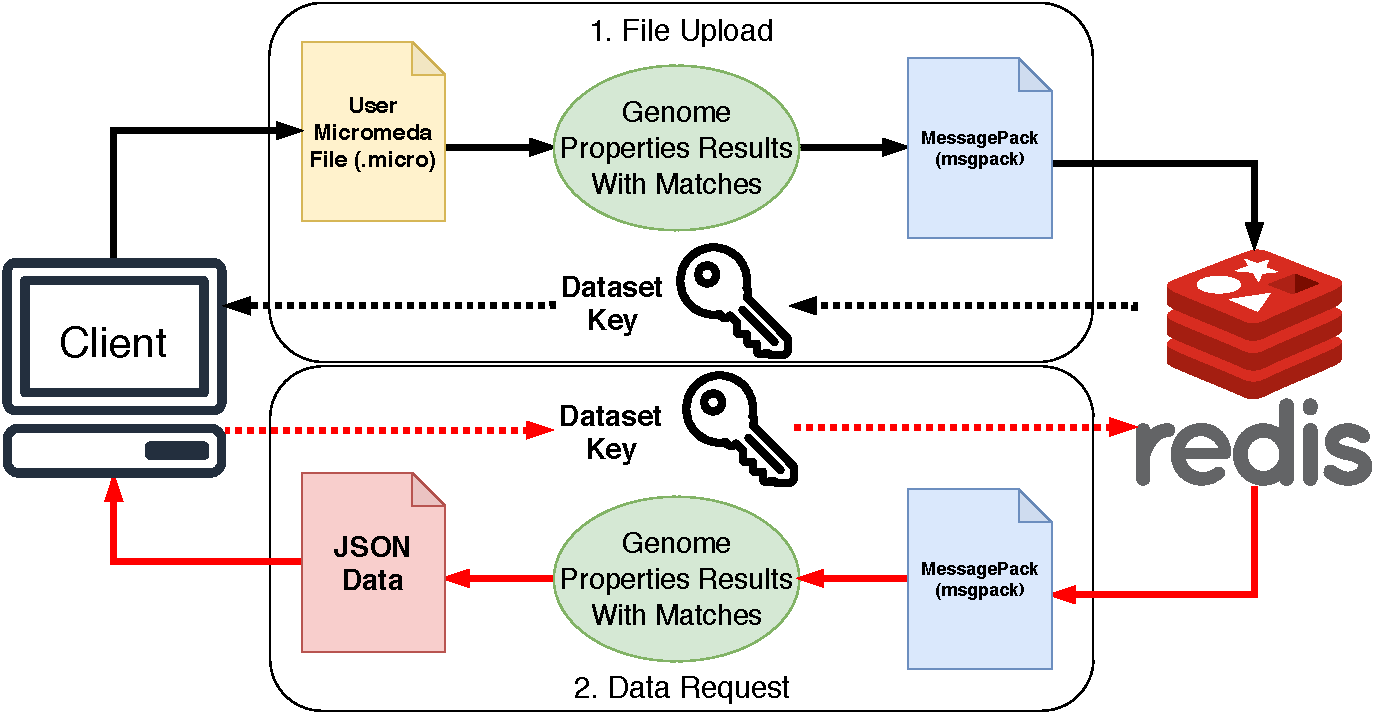
\includegraphics[width=\textwidth]{media/Micromeda-Server-Workflow.pdf}
	 \caption[How uploaded Micromeda files are cached to Redis by 
Micromeda-Server.]{\textbf{How uploaded Micromeda files are cached to Redis by 
Micromeda-Server.} The caching process involves the generation of 
GenomePropertiesResultsWithMatches objects for each uploaded file. These objects 
are cached in Redis and reconstituted between API calls. Micromeda-Server uses 
methods possessed by these reconstituted GenomePropertiesResultsWithMatches 
objects to produce responses that are sent back to a web client application. 
Each uploaded file is assigned a dataset key that is provided to the client. The 
client later uses this key to request data from a specific Micromeda file.}
	 \label{fig:micromeda-server-workflow}
\end{figure}

\begin{figure}[!ht]
  \centering
	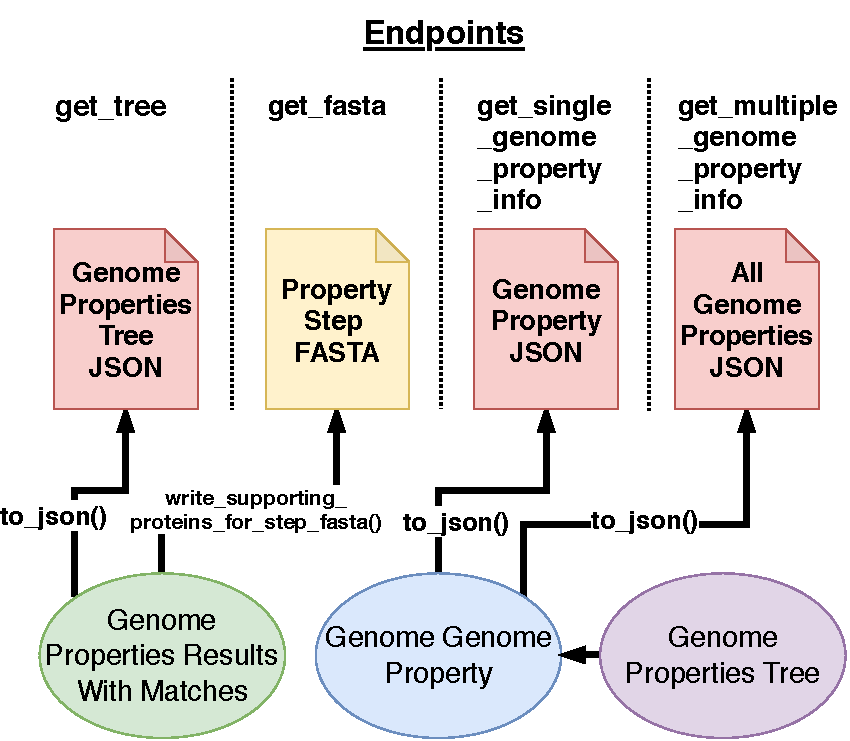
\includegraphics[width=0.7\textwidth]{media/Micromeda-Endpoints.pdf}
	 \caption[Endpoints that Micromeda-Server presents for accessing Genome 
Properties and Micromeda file data.]{\textbf{Endpoints that Micromeda-Server 
presents for accessing Genome Properties and Micromeda file data.} These 
endpoints return JSON documents and \gls{fasta} files that are generated using 
methods of GenomePropertiesResultsWithMatches objects, GenomeProperty objects, 
and GenomePropertiesTree objects.}
	 \label{fig:micromeda-endpoints}
\end{figure}

Each GenomePropertiesResultsWithMatches object cached to Redis is given a 
\gls{ttl} value \cite{gwertzman1996world} (see 
\href{http://en.wikipedia.org/wiki/Time_to_live}{en.wikipedia.org/wiki/Time\_to\_live}). 
Users can set this value for any period, such as minutes or days. After the 
\gls{ttl} of the cached object is exceeded, the object is flushed from the cache; the 
user will then have to re-upload their Micromeda file. The default \gls{ttl} 
used is six hours. During each \gls{api} request, if a dataset key is provided, 
the MessagePack-formatted GenomePropertiesResultsWithMatches object is grabbed 
from the cache and reconstituted into its original form (Fig. 
\ref{fig:micromeda-server-workflow}). During the \gls{api} call this 
reconstituted GenomePropertiesResultsWithMatches object's methods are used to 
supply data to the client  (Fig. \ref{fig:micromeda-server-workflow} and Fig. 
\ref{fig:micromeda-endpoints}). Further details on these endpoints are provided 
in Section \ref{endpoints}.

Micromeda files contain information about both assignments and supporting 
information used in their creation. This supporting information, such as protein 
sequences, can take up substantial disk space. Permanently storing such 
information would be prohibitive in terms of both hardware and maintenance 
costs. In response, Micromeda-Server was designed to store uploaded datasets 
temporarily. Micromeda-Server does not have a user login system \footnote{A user 
login system is very complex to build and maintain. Code for tracking user 
names, passwords, and emails must be generated. This user information must be 
stored in a cryptographically secured and anonymized database. Code for handling 
logins, logouts, and secure password changes would also have to be implemented. 
Having Micromeda file upload be anonymous drastically reduced the complexity of 
Micromeda-Server's development and future deployment.} and uploads to the server 
are done anonymously.

The number of simultaneous users that Micromeda-Server can support almost entirely depends on the server computer systems the software is run on and the deployment strategy used (see Section \ref{micromeda-server-deployments}).
Micromeda-Server is horizontally-scalable (see \href{https://en.wikipedia.org/wiki/Scalability#Horizontal_or_Scale_Out}{en.wikipedia.org/ wiki/Scalability\#Horizontal\_or\_Scale\_Out}), which means its performance can be 
improved by running multiple copies of the software across multiple server computer systems. On 
a single computer, the main bottleneck of Micromeda-Server is the processing 
power required to parse uploaded Micromeda files. For example, it can take 
several minutes for a Micromeda file containing information from forty bacterial 
genomes to be parsed and stored within Redis. This file parsing process can be 
parallelized across \gls{cpu} cores, with one core taking several minutes for 
parse each Micromeda file uploaded. Thus, the maximum number of simultaneous 
users who can upload Micromeda files in parallel is limited by the number of 
\gls{cpu} cores inside the server computer system on which Micromeda-Server is 
hosted. Once the contents of Micromeda files are stored in Redis, and 
information is being retrieved from this cache, the number of active users can 
be drastically increased as individual client endpoint \gls{http} requests take 
only a few \gls{cpu} cycles to complete. In terms of memory usage, a Micromeda 
file containing information from forty bacterial genomes only takes up a few 
hundred \gls{mb} of \gls{ram} once uploaded. A server with thirty-two \gls{gb} 
of \gls{ram} should support close to one hundred simultaneous clients requesting 
information from previously uploaded Micromeda files.

\section{Use of Redis for Dataset Caching} \label{redis-caching}

Python, due to limitations in its default cPython interpreter 
\cite{van1995python}, is only capable executing one compute thread 
\cite{saltzer1966traffic} (see 
\href{http://en.wikipedia.org/wiki/Thread_(computing)}{en.wikipedia.org/wiki/Thread\_(computing)}) 
at a time \cite{beazley2010understanding}. This limitation causes problems for 
web server \gls{api}s that are required to handle multiple requests from clients 
simultaneously. In response, the majority of Python web frameworks, which 
provide boilerplate code for writing \gls{api} endpoints, are designed to run 
multiple copies of the Python web server code, which each handle separate 
endpoint requests (Fig. \ref{fig:client-processing}). Flask is one such 
framework \cite{grinberg2018flask}. These codes are run in separate processes 
(see 
\href{http://en.wikipedia.org/wiki/Thread_(computing)\#Threads\_vs.\_processes}{en.wikipedia.org/wiki/ 
Thread\_(computing)\#Threads\_vs.\_processes}) and do not share a memory space 
(Fig. \ref{fig:client-processing}). Thus, any in-memory objects created for one 
\gls{api} request are not shared with the other parallel requests, which are 
being handled by different processes (Fig. \ref{fig:client-processing}). Also, 
there is no guarantee that subsequent \gls{api} requests from a single web 
client will be mapped repeatedly to the same \gls{api} server process (Fig. 
\ref{fig:client-processing}). This lack of mapping between subsequent requests 
causes a problem as a GenomePropertiesResultsWithMatches object created by the 
upload of a Micromeda file would be stored in one process and would not be 
available to other processes that future client \gls{http} requests may be 
mapped to (Fig. \ref{fig:client-processing}). One way of circumventing this 
process isolation issue is to store data to be shared between web server 
processes in an external process that is used as a cache (Fig. 
\ref{fig:micromeda-server-workflow} and Fig. \ref{fig:client-processing}). This 
way, all web \gls{api} processes have one place where they can request shared 
data. Micromeda-Server uses Redis as this caching process. Redis is a caching 
server that stores keyed Micromeda file data \gls{ram}. 

Micromeda-Server uses Redis to cache GenomePropertiesResultsWithMatches objects, 
in MessagePack format, for use by multiple request handling processes (Fig. 
\ref{fig:micromeda-server-workflow} and Fig. \ref{fig:client-processing}). 
Micromeda-Server generates these GenomePropertiesResultsWithMatches objects from 
Micromeda files uploaded to the server. During \gls{api} requests where a client 
requires data from a specific uploaded file, responding \gls{api} processes can 
each pull a MessagePack formatted GenomePropertiesResultsWithMatches object, 
representing the uploaded file, from the Redis cache. Subsequently, each 
GenomePropertiesResultsWithMatches object can be reconstituted within its 
process and its methods used to gather data for a \gls{api} request response 
(Fig. \ref{fig:micromeda-server-workflow} and Fig. \ref{endpoints}). Rapid 
serialization of MessagePack to GenomePropertiesResultsWithMatches objects 
allows for this design pattern (see Section \ref{msgpack}).

\begin{figure}[!ht]
  \centering
	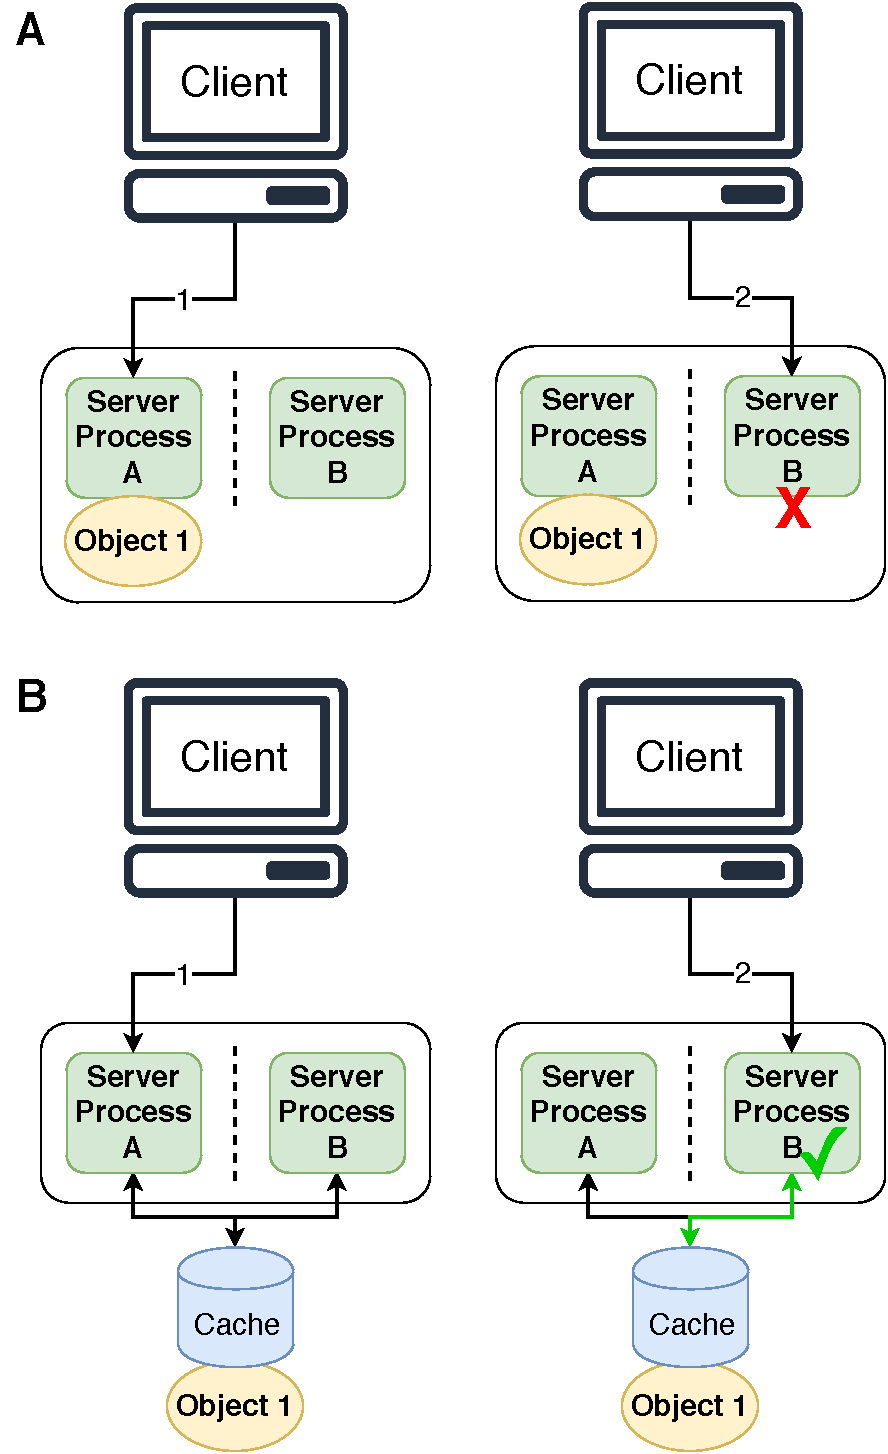
\includegraphics[width=0.50\textwidth]{media/Client-Processing.pdf}
	 \caption[How requests directed towards Python web endpoints are spread out across 
multiple processes and sharing data between these processes is 
difficult.]{\textbf{How requests directed towards Python web endpoints are spread 
out across multiple processes and sharing data between these processes is 
difficult.} (A) Processes cannot share in-memory objects directly due to 
operating system enforced process boundaries. (B) In order for data to be shared 
between request handling processes, it must be stored by a third central 
process, such as a cache or database.}
	 \label{fig:client-processing}
\end{figure}

\FloatBarrier
\section{Application Programming Interface Endpoints} \label{endpoints}

Micromeda-Server provides several endpoints for supplying web clients with 
information about individual genome properties and information from uploaded 
Micromeda files. These endpoints were written using the Flask Python web 
framework \cite{grinberg2018flask} and are represented by \textbf{clean 
\gls{url}s} (see 
\href{http://en.wikipedia.org/wiki/Clean_URL}{en.wikipedia.org/wiki/Clean\_URL}) 
where some information that would normally be stored as \gls{http} GET 
parameters are stored in the \gls{url} path (Fig. \ref{fig:endpoint-url}). Flask 
was chosen due to its simplicity as compared to more comprehensive frameworks 
such as Django \cite{holovaty2009definitive}. The endpoints also follow a 
\gls{rest} architecture \cite{fielding2000representational} (see 
\href{http://en.wikipedia.org/wiki/Representational_state_transfer}{en.wikipedia.org/wiki/Representational\_state\_transfer}). 
These endpoints and their implementation are summarized in Table 
\ref{tab:endpoints}, Fig. \ref{endpoints}, Fig. \ref{fig:endpoint-url}, and 
detailed in subsections below.

\begin{figure}[!ht]
  \centering
	
\includegraphics[width=0.95\textwidth]{media/Coloured-Endpoint.pdf}
     \caption[Example of a URL that a client would use to request information 
from Micromeda-Server.]{\textbf{Example of a \gls{url} that a client would use 
to request information from Micromeda-Server.} Micromeda-Server uses data held 
within \gls{url}s to figure out what information to return for a given 
\gls{http} request. The example \gls{url} depicted is used to download a 
\gls{fasta} file containing the top proteins (\textit{i}.\textit{e}., those with 
the lowest \gls{eval}  domains) that support GenProp0526 step one for dataset 
FXDABADS. The \gls{url} path variables are in blue and the \gls{http} GET 
parameters are in green. Note that the \gls{url} displayed is an example and does 
not point towards an active copy of Micromeda-Server or Micromeda-Client. Links 
to a demonstration of the client interface can be found in Section 
\ref{client-demo}.}
	 \label{fig:endpoint-url}
\end{figure}

\begin{longtable}{|p{1.6cm}|p{2.5cm}|p{1.4cm}|p{2.2cm}|p{2.2cm}|p{4cm}|}
\caption[Five endpoints of Micromeda's server component.]{Five endpoints of 
Micromeda's server component. By using these endpoints, clients can request data 
about individual genome properties, upload Micromeda files, and request 
information about stored assignment databases.}
\label{tab:endpoints}\\

\hline
\textbf{Python Function Name} & \textbf{Endpoint URL} & \textbf{HTTP Request 
Types} & \textbf{URL Path Variables} & \textbf{GET Parameter Variables} & 
\textbf{Return Value} \\ \hline
\endfirsthead
%
\multicolumn{6}{c}%
{{\bfseries Table \thetable\ continued from previous page}} \\
\hline
\textbf{Python Function Name} & \textbf{Endpoint URL} & \textbf{HTTP Request 
Types} & \textbf{URL Path Variables} & \textbf{GET Parameter Variables} & 
\textbf{Return Value} \\ \hline
\endhead
%
upload & /upload & GET, POST & None & None & \gls{json} containing a dataset key 
that can be used by future \gls{api} requests to access information from the 
uploaded Micromeda file \\ \hline
get\_tree & /genome \_properties \_tree & GET & None & dataset\_key (optional) & 
\gls{json} tree representing all properties in the current Genome Properties 
database with each node annotated with a list of YES, NO, PARTIAL assignments 
for each organism in a dataset \\ \hline
get\_single \_genome \_property \_info & /genome \_properties/ 
\textless{}string: property\_id\textgreater{} & GET & property\_id & None & 
\gls{json} containing information about a genome property such as a description 
of it and a list of equivalent records from other databases (\textit{e}.\textit{g}., \gls{kegg} 
\cite{kawashima2003kegg}, MetaCyc \cite{karp2002metacyc}) \\ \hline
get \_multiple \_genome \_property \_info & /genome \_properties & GET & None & 
None & \gls{json} array containing information about all genome properties in 
the database. Each property is given a description and a list of equivalent 
records from other databases (\textit{e}.\textit{g}., \gls{kegg}, MetaCyc) \\ \hline
get\_fasta & /fasta/ \textless{}string: property\_id\textgreater{}/ 
\textless{}int:step \_number\textgreater{} & GET & property\_id, step\_number & 
dataset\_key (optional), all (optional) & \gls{fasta} file containing either all or 
the top proteins (\textit{i}.\textit{e}., those with the lowest \gls{eval} domain annotations) 
supporting the existence of a given property step. A dataset key can be provided 
to specify a dataset \\ \hline
\end{longtable}

The \textbf{upload} endpoint accepts the client upload of a Micromeda file and 
returns a hexadecimal encoded \gls{uuid} key \cite{leach2005universally} (see 
\href{http://en.wikipedia.org/wiki/Universally_unique_identifier}{en.wikipedia.org/wiki/ 
Universally\_unique\_identifier}) to the client. After upload, the Micromeda 
file is parsed and transformed into a GenomePropertiesResultsWithMatches object. 
This object is then serialized to MessagePack using the object's 
\textbf{to\_msgpack} function (Table \ref{tab:genomepropertyresultswithmatches}) 
and the resulting binary is cached in Redis using the Redis Python library 
\cite{mccurdy_2019} (Fig. \ref{fig:micromeda-server-workflow}). During the 
previous process, a \gls{uuid}, to be used as a dataset key, is generated using 
Python's built in \gls{uuid} generation function \cite{PythonUUID}. This 
\gls{uuid} is used as the key for requesting the recently stored MessagePack 
serialization from the Redis cache (Fig. \ref{fig:micromeda-server-workflow}). 
Micromeda-Server returns the key to the client application in response to the 
file upload. The client can provide this key to other \gls{api} endpoints to 
receive data from the uploaded Micromeda file (Fig. 
\ref{fig:micromeda-server-workflow}). 

The \textbf{get\_tree} endpoint provides the client with a \gls{json} tree 
representing all properties and steps in Genome Properties database (Fig. 
\ref{fig:tree-json}). This tree represents parent-child relationships between 
properties. Step nodes are also attached to their parent genome property nodes 
and act as leaves (Fig. \ref{fig:tree-json}). Note that this endpoint returns a 
tree rather than a \gls{dag} (Fig. \ref{fig:tree-json}). In this tree, 
properties that would have had two parents in the Genome Properties \gls{dag} 
(Subsection \ref{micromeda-data-sources}) are duplicated (Fig. 
\ref{fig:tree-json}). Each property and step node in the tree is annotated by a 
list of assignments of support (\textit{i}.\textit{e}., YES, NO, or PARTIAL), one 
for each sample in a previously uploaded or default Micromeda file (Fig. 
\ref{fig:tree-json}). The \textbf{get\_tree} endpoint can take a 
\textbf{dataset\_key} \gls{http} GET parameter variable (Table 
\ref{tab:endpoints}). If a dataset key generated by the previous upload of a 
Micromeda file is assigned to this variable, then the assignments of support 
stored in the key's associated Micromeda file are returned. The dataset key is 
used to request a MessagePack formatted GenomePropertiesResultsWithMatches 
object, representing the uploaded Micromeda file, from the Redis cache. Once 
reconstituted, the GenomePropertiesResultsWithMatches object's \textbf{to\_json} 
method (Table \ref{tab:genomepropertyresultswithmatches}) is called to generate 
the tree \gls{json} provided by the endpoint. This newly built \gls{json} 
is returned to the client. If no dataset\_key is provided to the endpoint, then 
the default dataset GenomePropertiesResultsWithMatches object is used 
to generate the tree \gls{json} for the endpoint. The default dataset 
GenomePropertiesResultsWithMatches object is built from a default dataset 
Micromeda file that is provided to Microemda-Server during the tool's initial 
start up.

\begin{figure}[!ht]
  \centering
	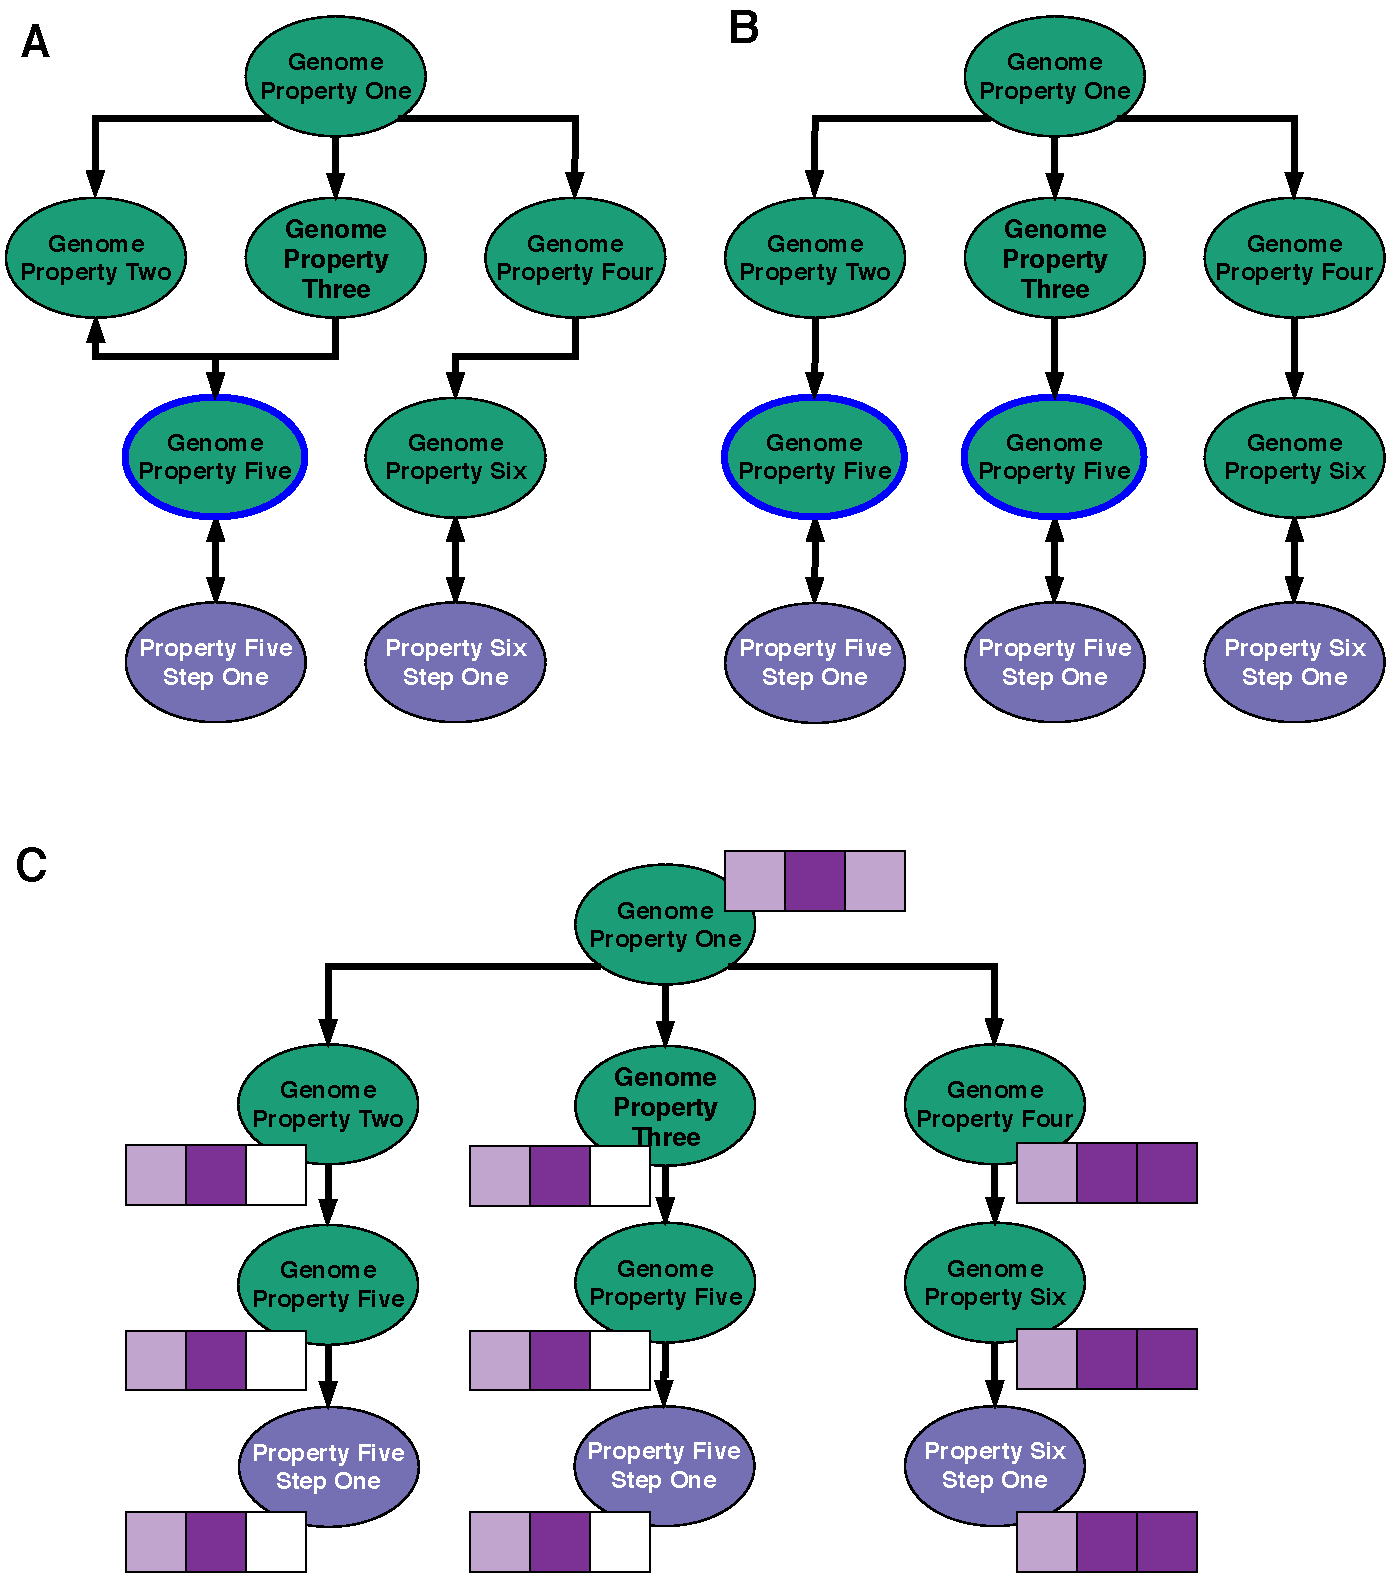
\includegraphics[width=0.70\textwidth]{media/Tree-JSON.pdf}
	 \caption[Comparison of the tree data structures returned by Micromeda-Server's 
Get\_Tree endpoint to the property DAG built by Pygenprop.]{\textbf{Comparison 
of the tree data structures returned by Micromeda-Server's Get\_Tree endpoint to 
the property \gls{dag} built by Pygenprop.} Unlike a \gls{dag} (A), a tree (B) 
cannot have branches that merge. Thus, the \gls{json} returned by the 
Get\_Tree can endpoint has some Genome Property nodes duplicated (B). In this 
JSON document, each node is tagged with a list of YES (Dark Purple), PARTIAL 
(Light Purple), and NO (White) assignments (C). Each assignment in this list 
belongs to a single organism in a dataset.}
	 \label{fig:tree-json}
\end{figure}

The \textbf{get\_single\_genome\_property\_info} endpoint takes a genome 
property identifier as a \gls{url} parameter (Table \ref{tab:endpoints}). This 
genome property identifier is used query for a matching GenomeProperty object 
(Section \ref{genome-property-class}), representing the property whose 
identifier is specified, from a global GenomePropertiesTree object (Section 
\ref{GenomePropertiesTree-Class}) created on Micromeda-Server's start up 
(Section \ref{server-workflow}). If found, this GenomeProperty object's 
\textbf{to\_json} method (Table \ref{tab:genome-property-object}) is called to 
create a \gls{json} document containing the property's information. The endpoint 
returns this document. The \gls{json} document contains the property's name, its 
description, and a list of equivalent records for the pathway that property 
represents found in other pathway databases (Table 
\ref{tab:genome-property-object}).

When the \textbf{get\_multiple\_genome\_property\_info} endpoint is called, the 
\textbf{to\_json} method (Table \ref{tab:genome-property-object}) is called for 
every GenomeProperty object (Section \ref{genome-property-class}) that is a 
child of the GenomePropertiesTree object (Section 
\ref{GenomePropertiesTree-Class}) created on Micromeda-Server start up. Each of 
the resulting \gls{json} strings generated is placed into a list within a single larger 
\gls{json} document, which is then returned by the endpoint. 

The \textbf{get\_fasta} endpoint is used to send the client a \gls{fasta} file 
containing protein sequences that support the existence of a property step 
across multiple organisms in a specific uploaded dataset. The \gls{url} path of 
requests to this endpoint includes the genome property identifier and step 
number of the property step whose protein matches should be included in the 
returned \gls{fasta} file. The returned FASTA file can either contain all 
proteins that support the existence of a property step or a subset of these 
supporting proteins, one per sample, that have the lowest \gls{eval} match to 
the InterPro domain that is used to identify the given property step. These 
proteins are known as the \textbf{``top"} hits. The contents of the returned 
file is controlled by the presence of a \gls{http} GET parameter called 
\textbf{all} (Fig. \ref{fig:endpoint-url}). If \textbf{all} is set to true, then 
a \gls{fasta} file containing all proteins that support a step is returned. 
Otherwise, a \gls{fasta} file containing only the lowest \gls{eval} proteins is 
returned. Like the \textbf{get\_tree} endpoint, the \textbf{get\_fasta} endpoint 
also accepts a \textbf{dataset\_key} \gls{http} GET parameter (Fig. 
\ref{fig:endpoint-url}). The value of this variable is used to reconstitute a 
GenomePropertiesResultsWithMatches object representing a previously uploaded 
Micromeda file (Fig. \ref{fig:micromeda-server-workflow}). This object's 
\textbf{write\_supporting\_proteins\_for\_step\_fasta} method (Table 
\ref{tab:genomepropertyresultswithmatches}) is used generate the \gls{fasta} 
file, which is sent to the client.

\section{Micromeda Server Performance} \label{micromeda-server-performance}

The performance of Micromeda's endpoints was tested using a Micromeda file 
generated from the protein sequences and InterProScan annotations of 
\textit{Chlorobium chlorochromatii} CaD3 (\gls{ncbitaxa}: 340177) and 
\textit{Pelodictyon luteolum} DSM 273 (\gls{ncbitaxa}:  319225). 
The performance metrics discussed in this section were recorded using Safari's 
(version 13; \href{http://apple.com/safari}{apple.com/safari}) Web Inspector.
When this file was sent to the \textbf{upload} endpoint of Micromeda-Server, it 
was parsed and added to the Redis cache in 11.3 s \textpm 2.0 s (\gls{n} = 3). 
The \textbf{get\_tree} endpoint could create a genome property tree from this 
cached Micromeda file in 9.4 s \textpm 4.0 s (\gls{n} = 3). The 
\textbf{get\_fasta} endpoint could generate a \gls{fasta} file with the top 
supporting proteins for GenProp0633 step number two in 33.0 ms \textpm 4.0 ms 
(\gls{n} = 10). A property information \gls{json} file could be generated for 
GenProp0633 by the \textbf{get\_single\_genome\_property\_info} endpoint in 7.0 
ms \textpm 2.0 ms (\gls{n} = 10). The 
\textbf{get\_multiple\_genome\_property\_info} endpoint can generate a 
\gls{json} information file for all properties in 23.0 ms \textpm 5.0 ms 
(\gls{n} = 10). The slow execution time of the \textbf{upload} and 
\textbf{get\_tree} endpoints caused latency in client application. For 
example, there was a noticeable delay in the rendering of visualizations in 
Micromeda's client application. Thus, the performance of these endpoints should 
be optimized. Potential optimizations to the endpoints are discussed in Section 
\ref{micromeda-server-improvements}.

\section{Micromeda Server Deployments} \label{micromeda-server-deployments}

It is common to deploy web servers in different configurations depending on the 
expected request volume. Three deployment strategies of increasing size are 
discussed below. 

If a user wishes to install and run Micromeda-Server on their desktop or laptop 
and only needs to visualize one dataset at a time, then a very simplified 
deployment strategy can be used (Fig. \ref{fig:micromeda-small-deploy}). This 
deployment, called a single-user deployment, uses Flask's built-in development 
\gls{http} server to respond to requests. The server is activated when 
Micromeda-Server's Python script is run directly from a \gls{cli}. This 
single-user deployment is slow and can only handle requests from a single 
client. In this configuration, the upload endpoint is turned off, and Redis is 
not used. As a result, users cannot upload Micromeda files. Instead, 
Micromeda-Server gets its assignment data from a single default Micromeda file 
stored on disk (Fig. \ref{fig:micromeda-small-deploy}). This deployment method 
is similar to the one used by Anvio's \gls{mags} visualization and refinement 
server \cite{eren2015anvi}. The single-user deployment configuration is also 
useful to developers who want to test newly developed features or bug fixes.

\begin{figure}[!ht]
  \centering
	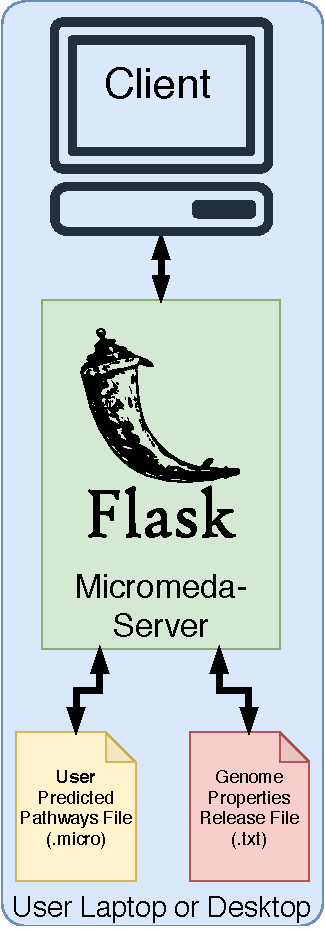
\includegraphics[width=0.20\textwidth]{media/micromeda-simple-deployment.pdf}
	 \caption[How Micromeda-Server would be deployed to support a development or 
single-user environment.]{\textbf{How Micromeda-Server would be deployed to 
support a development or single-user environment.} In this deployment style, 
Micromed-Server uses Flask's builtin \gls{http} server, a genomeProperties.txt 
file, and a server-side Micromeda file. However, this deployment style 
encounters problems when used by multiple users because only a single copy of 
the Python Flask code is run at a time.}
	 \label{fig:micromeda-small-deploy}
\end{figure}

If a user requires Micromeda-Server to handle multiple users simultaneously, 
such as would be the case if the software was installed on a server computer 
system, a larger deployment must be used (Fig. 
\ref{fig:micromeda-medium-deploy}). This deployment type, called a multi-user 
deployment, adds additional software layers that increase Micromeda-Server's 
scalability. As discussed in previous sections, multiple copies of 
Micromeda-Server's Python code must be run simultaneously to handle multiple 
client requests. This technique is done by putting the Micromeda-Server under 
the command of a master \gls{http} server that can route traffic to multiple 
copies of the Python Flask code running separate processes (Fig. 
\ref{fig:micromeda-medium-deploy}). Examples of such master \gls{http} servers 
are Apache \cite{fielding1997apache} and Nginx \cite{reese2008nginx} \gls{http} 
servers. These master servers handle the parsing of \gls{http} requests. In 
addition to the master server, a middleware component, such as\gls{uwsgi} 
\cite{2019uwsgi} or gunicorn \cite{chesneau_2018}, must also be used. Redis is 
used to cache GenomePropertiesResultsWithMatches objects between requests in 
this deployment type. All components of Micromeda-Server deployed on the same 
server computer system (Fig. \ref{fig:micromeda-medium-deploy}).

\begin{figure}[!ht]
  \centering
	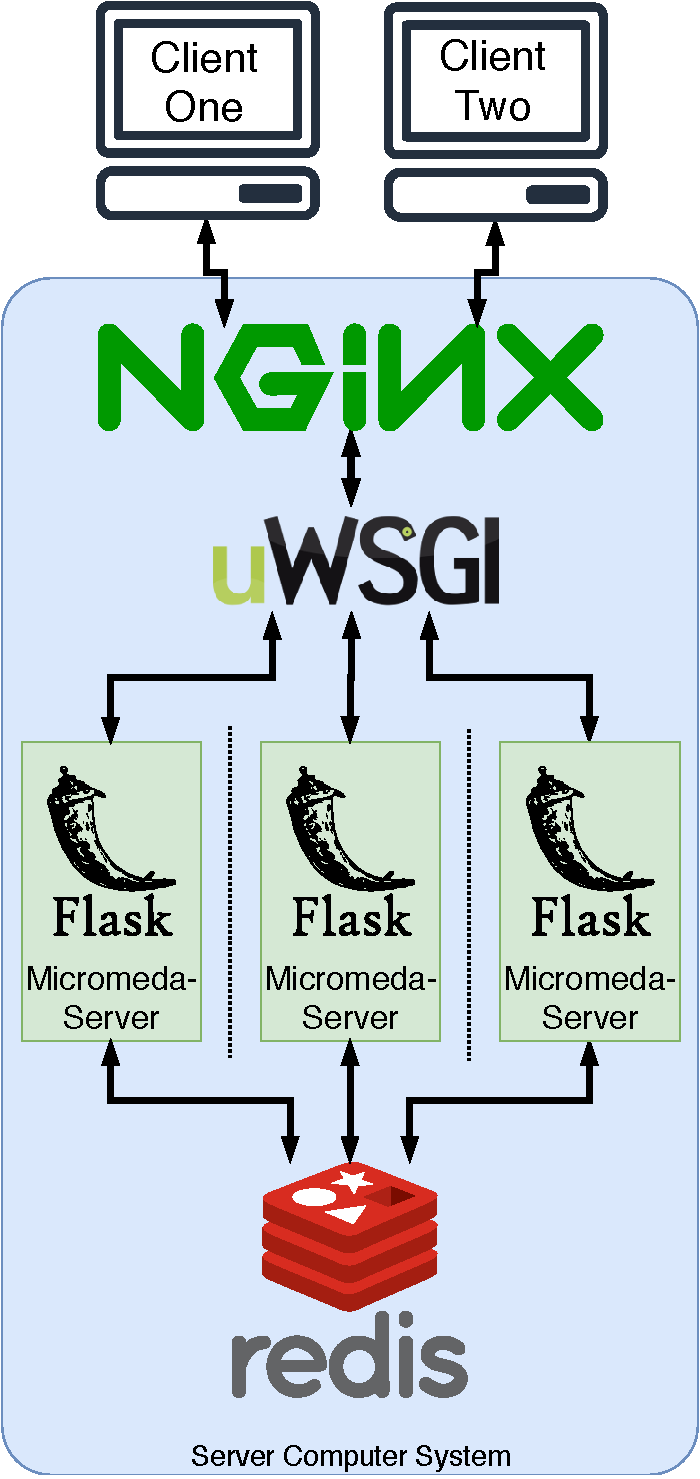
\includegraphics[width=0.30\textwidth]{media/micromeda-medium-deployment.pdf}
	 \caption[How Micromeda-Server would be deployed to support multiple users 
using a single server computer system.]{\textbf{How Micromeda-Server would be 
deployed to support multiple users using a single server computer system.} When 
deployed to handle the traffic of multiple clients, Multiple other types of 
software must support Micromed-Server. Multiple copies of the application's 
Python code are run simultaneously to handle multiple clients. Redis is used to 
provide shared data between these processes. A \gls{uwsgi} middleware component 
is used to connect these copies to a high performance \gls{http} server, such as 
Nginx, that can handle high web traffic volumes. The genomeProperties.txt files 
and default Micromeda files are still used in this deployment style but were 
omitted from the diagram for simplicity.}
	 \label{fig:micromeda-medium-deploy}
\end{figure}

\pagebreak

For a large number of simultaneous users, Micromeda-Server may need to be scaled 
horizontally across multiple servers (Fig. \ref{fig:micromeda-large-deploy}). 
This deployment type is called a multi-server deployment. The scaling is 
facilitated by placing a load balancer 
(\href{http://en.wikipedia.org/wiki/Load_balancing_(computing)}{en.wikipedia.org/wiki/ 
Load\_balancing\_(computing)}) out front of multiple copies of the multi-user 
deployment running on separate server computer systems (Fig. 
\ref{fig:micromeda-large-deploy}). Redis can also be run on a separate server 
computer system or computing cluster (Fig. \ref{fig:micromeda-large-deploy}). 
Such multiple server deployment strategies can be scaled horizontally by adding 
new server computer systems to the deployment (Fig. 
\ref{fig:micromeda-large-deploy}). These new server computer systems allow for 
increases in request volume.

\begin{figure}[!ht]
  \centering
	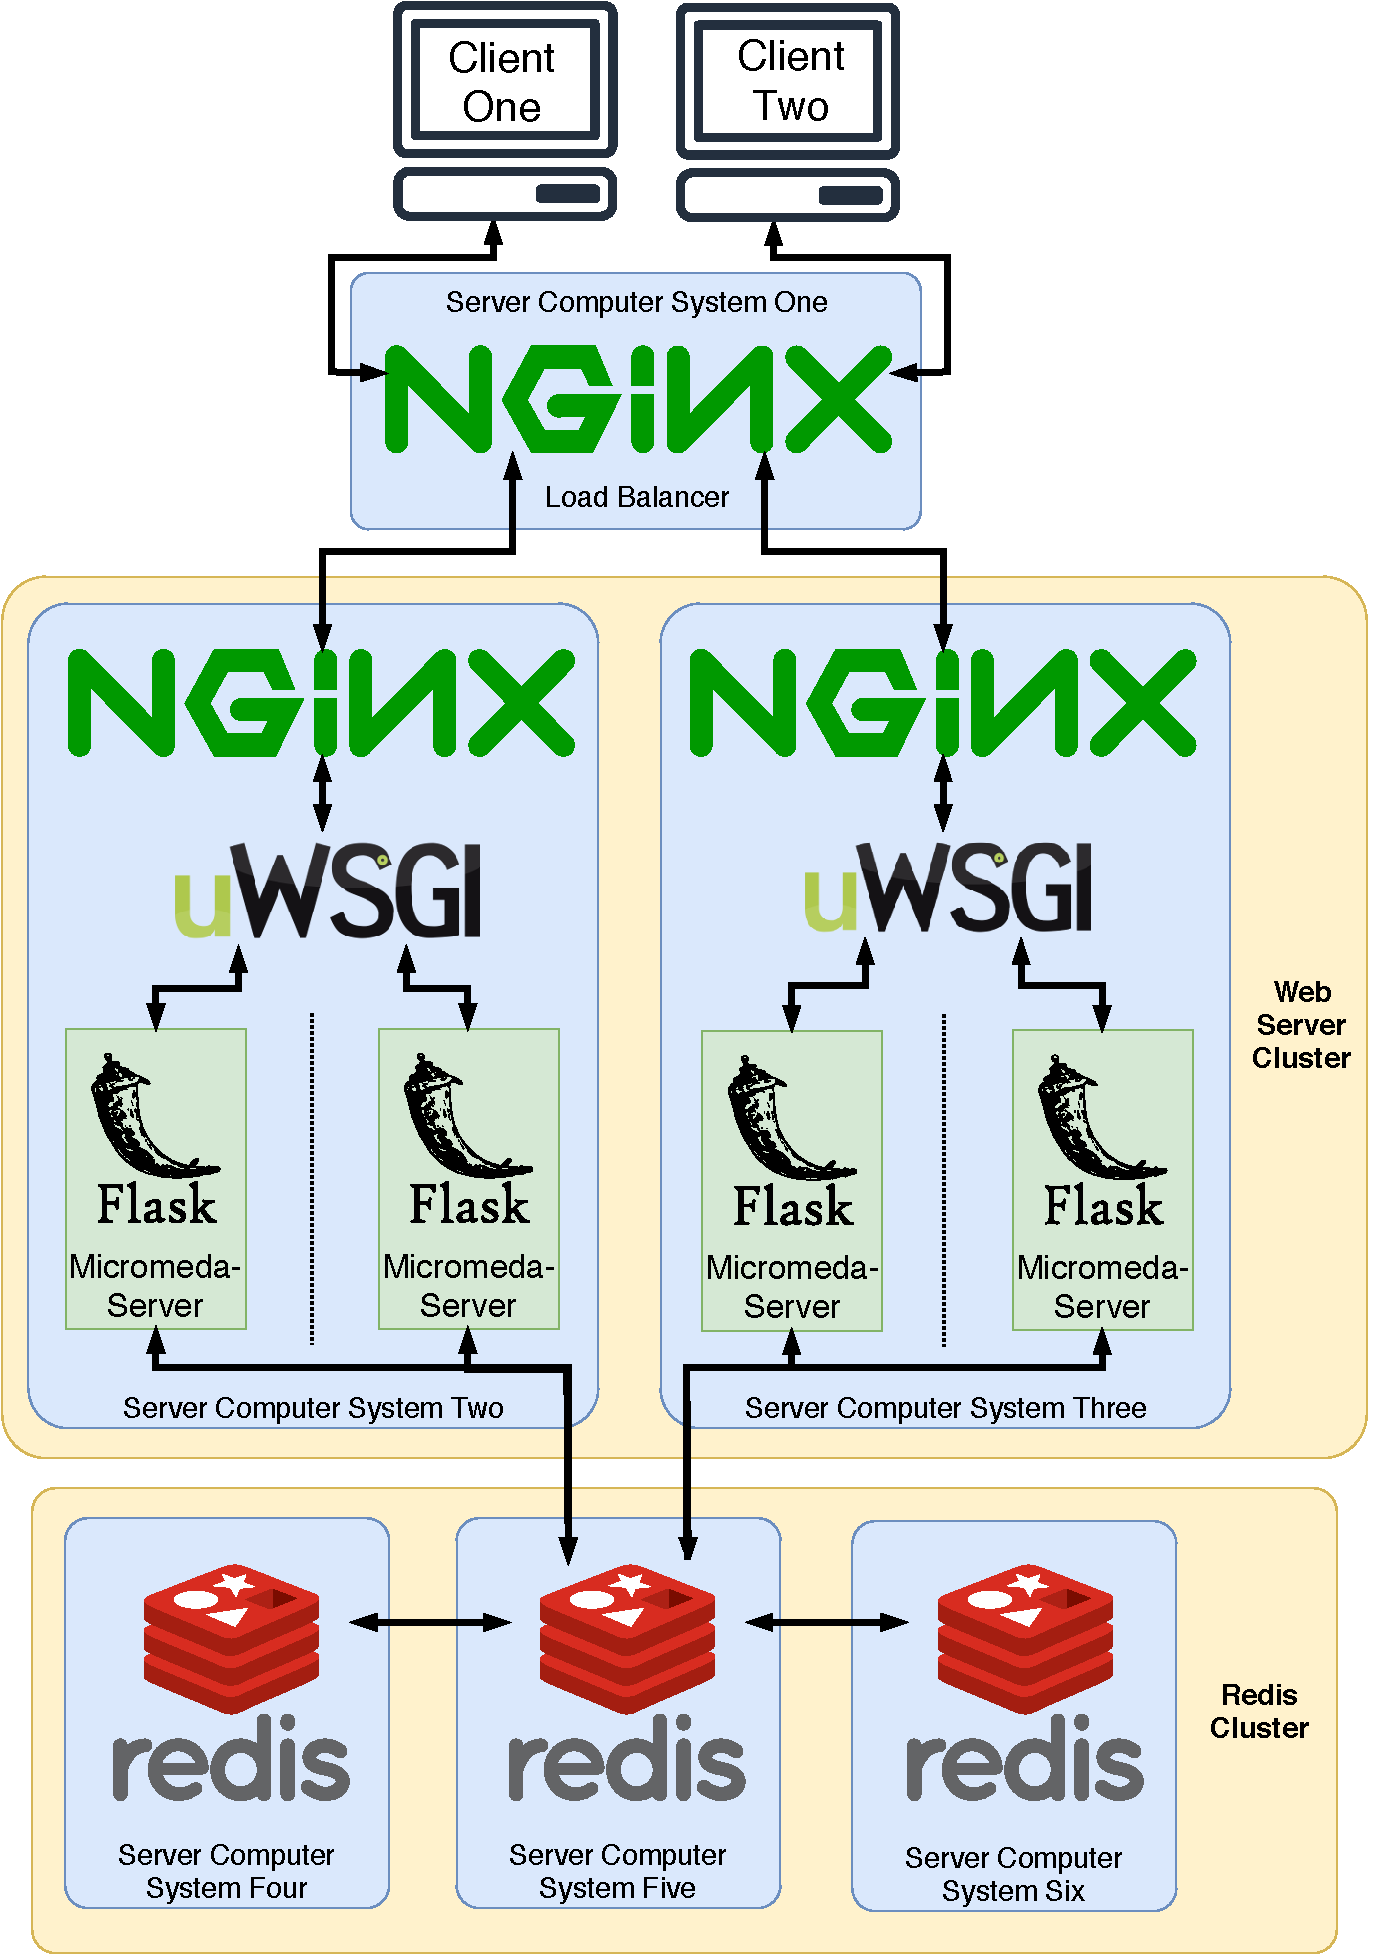
\includegraphics[width=0.60\textwidth]{media/micromeda-heavy-deployment.pdf}
	 \caption[How Micromeda-Server would be deployed to support multiple users 
using a cluster of computer systems.]{\textbf{How Micromeda-Server would be 
deployed to support multiple users using a cluster of computer systems.} When 
Micromeda is required to scale to handle hundreds or thousands of simultaneous 
users, its workload must be spread out across multiple caching and web server 
computer systems. Each node in the web server cluster runs additional copies of 
Micromeda-Server and supporting software. The performance of such deployments 
can be increased by adding hardware to either the caching or web server 
clusters. A copy of the genomeProperties.txt file and default Micromeda file 
would be stored in each server computer system in the web server cluster. These 
file have been omitted from the diagram for simplicity.}
	 \label{fig:micromeda-large-deploy}
\end{figure}

Various cloud computing corporations have developed \gls{paas} 
\cite{lawton2008developing} products (see 
\href{http://en.wikipedia.org/wiki/Platform_as_a_service}{en.wikipedia.org/wiki/Platform\_as\_a\_service}) 
that help users scale Python web applications without having to spend time 
setting up complex multi-server deployments. These \gls{paas}, such as Google 
App Engine (\href{http://cloud.google.com/appengine}{cloud.google.com/ 
appengine}) or Heroku (\href{http://heroku.com}{heroku.com}), provide the 
simplicity of a single-user deployment with the scalability of multi-server 
deployment. When a developer's code is deployed to a \gls{paas}, the resulting 
deployment, called a \gls{paas} deployment, provides attributes of both 
single-user deployments and multi-server deployments. For example, developers 
are only required to upload their Python code files to the platform and, 
subsequently, the platform will automate the rest of the deployment process. For 
example, the \gls{paas} will create load balancers and multiple copies of 
request handling Python processes automatically. Such platforms perform scaling 
tasks in the background and invisibly to the developer who uploaded the code.

\FloatBarrier
\section{Future Improvements} \label{micromeda-server-improvements}

Micromeda-Server currently possesses endpoints that provide all the information 
needed by Micromeda’s web-based visualization client (see Section 
\ref{endpoints}). One endpoint provides an annotated Genome Properties tree that 
includes information about both the structure of the Genome Properties database 
and assignments of supports for properties and steps. Other endpoints offer 
detailed information about individual properties and steps, and allow for the 
download of protein sequences that support property steps. In addition to the 
existing endpoints, new endpoints could be made that would provide new data for 
future versions of this client, allowing it to have expanded functionality. 
Performance optimizations for the existing endpoints could also be made, which 
could reduce latency in the client’s \gls{ui} by reducing the time spent waiting 
for responses from Micromeda-Server. Improvements to Micromeda-Server’s existing 
endpoints and a potential new endpoint are discussed below.

\subsection{Improving Performance of the Upload Endpoint}

The \textbf{upload} endpoint takes a Micromeda file and saves the file's 
contents to a Redis cache. This endpoint was shown to have poor performance (see 
Section \ref{micromeda-server-performance}) and should be optimized to be more 
responsive. Most of the performance problems with this endpoint can be 
attributed to the performance of parsing Micromeda files into 
GenomePropertiesResultsWithMatches objects using the 
\textbf{load\_assignment\_caches\_from\_database \\ \_with\_matches} function of 
Pygenprop's results module. The performance of this function was also weak (see 
Subsection \ref{micromeda-file-performance}). Performance improvements to this 
function are discussed in detail in Subsection 
\ref{improving-pygenprop-performance}. The performance optimizations recommended 
in that section should be adopted and will drastically improve the performance 
of the upload endpoint.

\subsection{Improving Performance of the Get\_Tree Endpoint and Building 
Endpoints for Returning Property and Step Assignments} 
\label{assignment-endpoints}

The \textbf{get\_tree} endpoint sends \gls{json} to the client that contains 
both property tree and assignment data. This \gls{json} is generated by calling 
a GenomePropertiesResultsWithMatches object's \textbf{to\_json} method. This 
method is known to have speed issues (see Subsection \ref{matches-performance} 
and Section \ref{micromeda-server-performance}) due to the method having to 
insert assignments into the \gls{json} tree one at a time, rather than in batch. 
This speed issue could be addressed by reconfiguring Micromeda-Server's 
\textbf{get\_tree} endpoint to no longer output a tree annotated by property 
assignments. Instead, new endpoints could be built that return step and property 
assignments separately (Fig. \ref{fig:new_endpoints}). New methods of 
GenomePropertiesResultsWithMatches objects would have to be developed to 
generate \gls{json} for these new endpoints (Section 
\ref{improving-pygenprop-performance}). The code for generating the property 
tree \gls{json} could be moved to the GenomePropertiesTree class (Fig. 
\ref{fig:new_endpoints}).

Caching the \gls{json} generated by endpoints in Redis could also improve these 
endpoint's performance. On subsequent \gls{api} calls, the cached data could be 
recalled from Redis and immediately returned to the client instead of being 
regenerated with every \gls{api} call. For example, only having to generate a 
property tree once procedurally would significantly improve endpoint 
performance.

\begin{figure}[!ht]
  \centering
	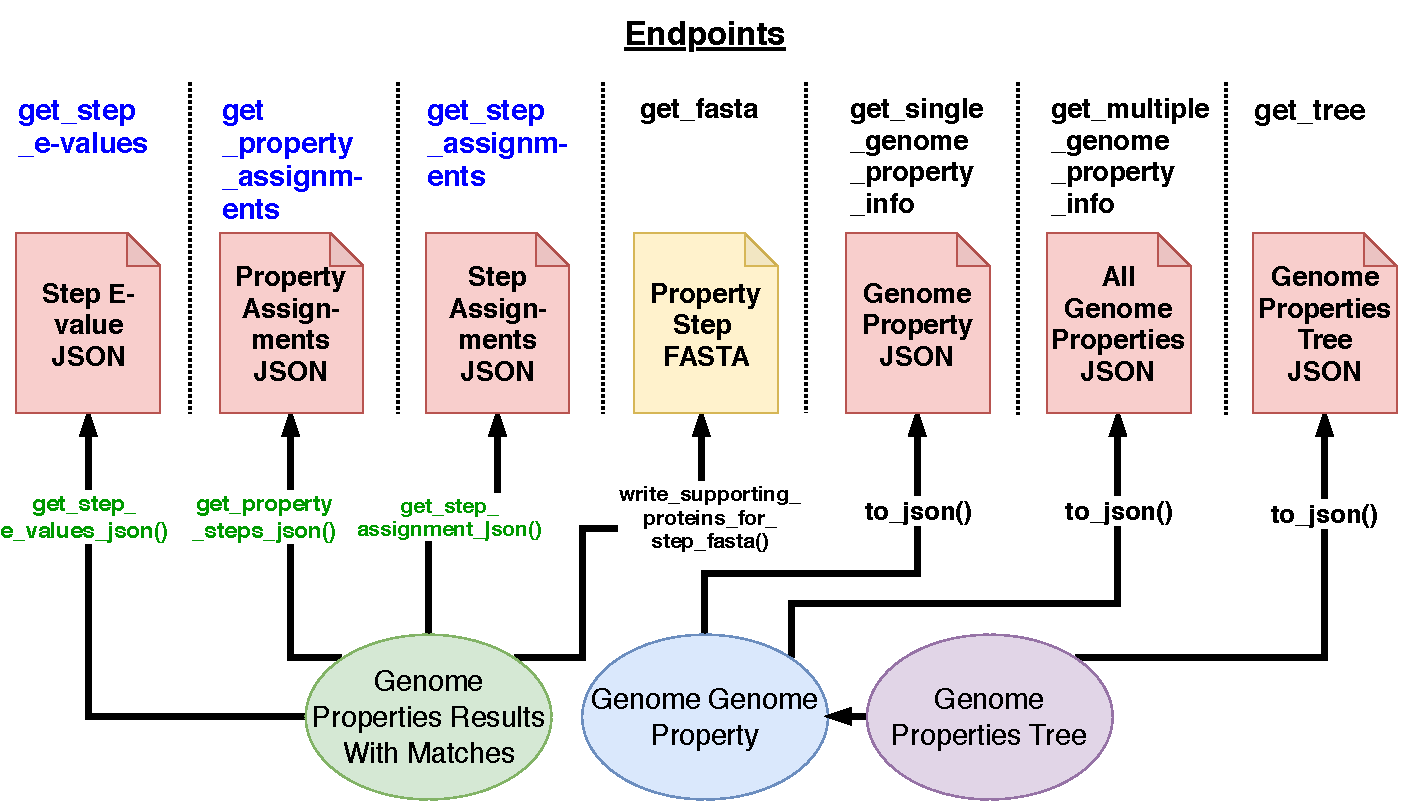
\includegraphics[width=\textwidth]{media/micromeda-server-new-endpoints.pdf}
	 \caption[New endpoints that could be added to Micromeda-Server to allow for 
expanded client functionality.]{\textbf{New endpoints that could be added to 
Micromeda-Server to allow for expanded client functionality.} These endpoints 
(blue) would return step assignments, step supporting information, and property 
assignments. New endpoints would be supported by new \gls{json} generating 
methods of GenomePropertiesResultsWithMatches objects (green).}
	 \label{fig:new_endpoints}
\end{figure}

\subsection{Creation of an Endpoint for Returning Domain Annotations Supporting 
Property Steps} \label{e-value-endpoint}

Micromeda files not only contain property and step assignments for a set of 
organisms but also contain additional information such as domain annotations and 
proteins sequences that support the existence of property steps. 
Micromeda-Server currently provides an endpoint for accessing protein sequences 
that support steps (see Section \ref{endpoints}). However, there are 
no endpoints for accessing the stored InterProScan annotations of these 
proteins. Specifically, these annotations contain \gls{eval} scores representing 
how closely the domain in the protein matches to a model of a representative 
domain in a protein database (see Subsection \ref{micromeda-data-sources}). The 
\gls{eval} scores for these domains may be useful to client visualizations that 
compare not only the presence and absence of proteins that support property 
steps but also compare how close these matches are to existing domain models. 
Thus, it may be useful to create a new endpoint that returns domain annotation 
\gls{eval} scores for domains that support property steps (Fig. 
\ref{fig:new_endpoints}). This endpoint could generate its data from the 
\textbf{step\_matches} DataFrame of reconstituted 
GenomePropertiesResultsWithMatches objects.

\section{Summary} \label{server-summary}

The creation of web server \gls{api}'s for accessing information about 
biochemical pathways, and even the precalculated presence and absence of these 
pathways across organisms, is quite common 
\cite{wu2006kobas,moriya2010pathpred,pireddu2006path,vallenet2009microscope,aziz2008rast,takami2016automated,moriya2007kaas,chou2009fmm}. 
Indeed, such web \gls{api}s have been developed by both the creators of 
\gls{kegg} \cite{kawashima2003kegg} and MetaCyc \cite{karp2013data}, not only 
for these database's web client applications but also for academic use. A web 
server has also been built for Genome Properties database website 
\cite{richardson2018genome} that is hosted by the \gls{ebi}. However, the 
server's \gls{api} is not publicly available and is only designed to support the 
Genome Properties website. The \gls{kegg}, MetaCyc, and Genome Properties 
website all contain precalculated pathway annotations for sets of reference 
organisms \cite{kanehisa2000kegg,karp2002metacyc,karp2013data}. Many pathway 
annotation web sites such as \gls{fmm} \cite{chou2009fmm}, \gls{kaas} 
\cite{moriya2007kaas} and \gls{maple} \cite{takami2016automated} can pathway 
annotate user-supplied genomes uploaded in \gls{fasta} format 
\cite{pearson19905}. Such annotation servers are complex to build and host due 
to the relative computational complexity of scanning for genes that support the 
existence of pathway steps. In contrast, the Genome Properties website allows 
for the upload of user-created InterProScan annotation files. The creation of 
such annotations files pushes the most computationally complex part of the 
Genome Properties pipeline, domain annotation, off onto end-users 
\cite{richardson2018genome}. As discussed in Subsection 
\ref{why-micromeda-files}, Micromeda-Server follows a similar approach. However, 
unlike the Genome Properties website, Micromeda-Server takes the upload of 
Micromeda files. Micromeda files allow the upload of datasets consisting of 
pathway annotations from multiple genomes simultaneously, unlike other pathway 
servers, which often require uploading genomes or InterProScan annotations for 
organisms one at a time. Also, because Micromeda files contain protein sequences 
that support pathway annotations, Micromeda-Server can present these sequences 
for download by users, which is a feature of few other pathway annotation servers 
currently possess. With the avoidance of computationally complex annotation 
steps and a variety of horizontally scalable deployment options, 
Micromeda-Server should provide a reliable and sustainable \gls{api} for 
Micromeda's client application.